\documentclass[11pt,a4paper]{article}

% ── Packages ──────────────────────────────────────────────────────────
\usepackage[utf8]{inputenc}
\usepackage[T1]{fontenc}
% Font: use default Computer Modern
\usepackage[english]{babel}
\usepackage[margin=2.2cm,top=2.4cm,bottom=2.4cm]{geometry}
\usepackage{graphicx}
\usepackage{xcolor}
\usepackage{hyperref}
\usepackage{enumitem}
\usepackage{booktabs}
\usepackage{tabularx}
\usepackage{titlesec}
\usepackage{fancyhdr}
\usepackage{float}
\usepackage{multicol}
\usepackage{parskip}
\usepackage{caption}
\usepackage{tikz}
\usetikzlibrary{shapes.geometric, arrows.meta, positioning, fit, backgrounds}

% ── Colors ────────────────────────────────────────────────────────────
\definecolor{rteblue}{HTML}{1B3A5C}
\definecolor{rtecyan}{HTML}{00A3E0}
\definecolor{rtegray}{HTML}{5A6872}
\definecolor{lightbg}{HTML}{F0F4F8}
\definecolor{accentgreen}{HTML}{2E8B57}

% ── Hyperref setup ────────────────────────────────────────────────────
\hypersetup{
  colorlinks=true,
  linkcolor=rteblue,
  citecolor=rteblue,
  urlcolor=rtecyan,
  pdfauthor={ST7 Cohort -- CentraleSupélec},
  pdftitle={LLM-Based Log Contextualization for Smart Grid Operations},
}

% ── Header/Footer ─────────────────────────────────────────────────────
\pagestyle{fancy}
\fancyhf{}
\fancyhead[L]{\small\textcolor{rtegray}{ST7 Smart Cities -- CentraleSupélec}}
\fancyhead[R]{\small\textcolor{rtegray}{February 2026}}
\fancyfoot[C]{\small\thepage}
\renewcommand{\headrulewidth}{0.4pt}

% ── Section styling ───────────────────────────────────────────────────
\titleformat{\section}{\large\bfseries\color{rteblue}}{\thesection}{0.8em}{}
\titleformat{\subsection}{\normalsize\bfseries\color{rteblue!80!black}}{\thesubsection}{0.6em}{}
\titlespacing*{\section}{0pt}{1.2em}{0.5em}
\titlespacing*{\subsection}{0pt}{0.8em}{0.3em}

% ── Compact lists ─────────────────────────────────────────────────────
\setlist{nosep, leftmargin=1.5em}

\begin{document}

% ══════════════════════════════════════════════════════════════════════
% TITLE PAGE
% ══════════════════════════════════════════════════════════════════════
\begin{titlepage}
\centering
\vspace*{1.5cm}

{\Huge\bfseries\color{rteblue} LLM-Based Log Contextualization\\[0.3em] for Smart Grid Operations\par}

\vspace{0.8cm}
{\Large\color{rtegray} Transforming Unstructured Operational Data\\into Actionable Insight\par}

\vspace{1.5cm}


\begin{tikzpicture}
  \fill[rteblue!10, rounded corners=8pt] (-4,-0.8) rectangle (4,0.8);
  \node[text=rteblue, font=\large\bfseries] at (0,0.15) {ST7 Smart Cities};
  \node[text=rtegray, font=\normalsize] at (0,-0.3) {CentraleSupélec -- March 2026};
\end{tikzpicture}

\vspace{1.5cm}

\begin{tabular}{rl}
  \textbf{Supervision:} & Noureddine Henka (RTE France) \\
  \textbf{Project Team:} & ST7 group \\
  \textbf{Academic Frame:} & Smart Cities Module \\
\end{tabular}

\vfill

{\small\color{rtegray} Project Report -- Asynchronous Multi-Agent Platform for Grid Log Analysis}
\end{titlepage}

% ══════════════════════════════════════════════════════════════════════
% BODY
% ══════════════════════════════════════════════════════════════════════

\section{Introduction and Context}

RTE (Réseau de Transport d'Électricité) operates the French high-voltage transmission grid, ensuring the continuous delivery of electricity from producers to consumers across the country. With the accelerating integration of intermittent renewable energy sources such as solar and wind, grid operations have become significantly more complex, requiring faster and more precise balancing decisions.

Grid operators rely on daily operational synthesis reports---dense, multi-page PDF documents written in French---to track incidents, outages, equipment faults, and market adjustments. These reports follow heterogeneous formatting conventions, may contain scanned pages and hand-annotated schematics, and demand substantial time to read and triage manually. During high-pressure operational periods, the latency introduced by manual reading is operationally unacceptable.

This project addresses the challenge by building an \textbf{asynchronous multi-agent platform} that automatically ingests these PDF logs, extracts structured incident data, classifies and prioritizes incidents by severity, and produces a decision-ready analysis report enriched with domain knowledge via Retrieval-Augmented Generation (RAG). The platform transforms hours of manual reading into actionable, RAG-grounded markdown output delivered in seconds.

The project was carried out within the ST7 Smart Cities module at CentraleSupélec under the supervision of RTE France, with three formal deliverables: a state-of-the-art review on LLMs and RAG for operational contextualization, a fully implemented pipeline with prompt engineering and RTE log integration, and multi-modal processing capabilities for handling figures, tables, and schematics.

\section{State of the Art: LLMs and RAG for Grid Operations}

Large Language Models such as GPT-4 and Mistral have demonstrated strong capabilities in information extraction and zero-shot reasoning, acting as general-purpose logic engines. However, applying them directly to domain-specific operational contexts like electricity grid management presents a fundamental limitation: pure LLMs lack native knowledge of internal grid codes, RTE-specific procedures, and operational terminology, which makes them prone to hallucination when generating domain-specific analysis.

Retrieval-Augmented Generation (RAG) addresses this gap by injecting retrieved domain knowledge directly into the LLM prompt at inference time. The approach follows a four-step cycle: the user prompt is sent to a vector database containing indexed RTE procedures and historical documents; relevant chunks are retrieved based on semantic similarity; these chunks are merged into an enriched prompt; and the LLM generates a factually grounded response. This architecture guarantees domain-aware generation without requiring expensive model fine-tuning, making it suitable for operational deployment where procedures evolve frequently.

The literature review conducted as part of this project confirmed that the combination of deterministic preprocessing (rule-based extraction) with selective LLM invocation offers the best trade-off between reliability, auditability, and coverage of edge cases in document formats.

\section{System Architecture}

The platform follows a clear separation between a \textbf{frontend} user interface and a \textbf{backend} processing engine, connected through a RESTful API with asynchronous job management.

\subsection{Frontend (Next.js Dashboard)}

The frontend is a Next.js (React) application providing a PDF upload interface, real-time job status polling via \texttt{GET /api/jobs/\{job\_id\}}, stage-by-stage pipeline progress visualization (collector, preprocessing, incident, analysis), markdown report rendering, and an LLM diagnostics panel exposing provider, model, latency, parse status, and raw output preview. Users can export the generated analysis as Markdown, plain text, or print-to-PDF directly from the interface.

\subsection{Backend (FastAPI Engine)}

The backend is a FastAPI service that handles file validation and storage, persistent SQL-based job tracking (PostgreSQL in production, SQLite for development), the full multi-agent orchestration pipeline executed asynchronously, and intermediate artifact persistence for traceability.

\subsection{Orchestrator and Job Processor}

The orchestrator is the central coordinator guaranteeing strict sequential execution of the four pipeline agents: \texttt{collector $\rightarrow$ preprocessing $\rightarrow$ incident $\rightarrow$ analysis}. It emits stage updates (running, completed, failed) for real-time frontend visibility and supports partial results when early stages succeed but a later stage fails, ensuring maximum information recovery.

The job processor wraps the orchestrator with production-grade concerns: concurrency control via semaphore, configurable timeout and retry policies, and persistent job state updates (queued, running, completed, partial, failed). This separation keeps the orchestration logic clean while ensuring reliable asynchronous execution.

\subsection{Data and Knowledge Layer}

Persistent storage uses PostgreSQL for job metadata, stage events, and artifacts. A lightweight JSON-based vector store (with ChromaDB as future target) provides RAG retrieval, seeded from historical RTE PDF documents. Uploaded files are stored durably on the filesystem with SHA-256 content hashing enabling deduplication.

\begin{figure}[H]
\centering
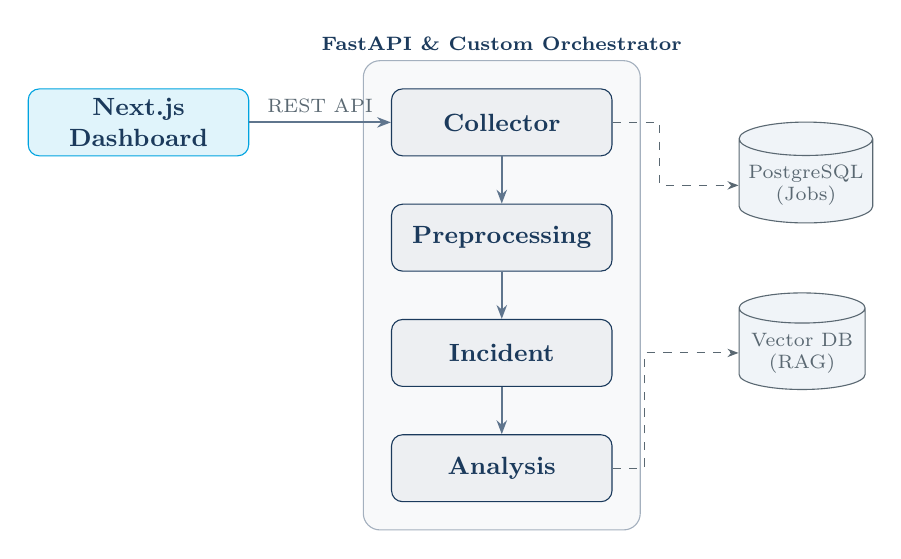
\begin{tikzpicture}[
  node distance=0.6cm and 1.2cm,
  box/.style={rectangle, draw=rteblue, fill=rteblue!8, rounded corners=4pt,
              minimum height=0.85cm, minimum width=2.8cm, align=center,
              font=\small\bfseries, text=rteblue},
  db/.style={cylinder, draw=rtegray, fill=lightbg, shape border rotate=90,
             aspect=0.25, minimum height=0.9cm, minimum width=1.6cm,
             font=\scriptsize, text=rtegray, align=center},
  arr/.style={-{Stealth[length=5pt]}, thick, rteblue!70},
  darr/.style={-{Stealth[length=4pt]}, dashed, rtegray},
]
  % Frontend
  \node[box, fill=rtecyan!12, draw=rtecyan] (fe) {Next.js\\Dashboard};
  % Backend agents
  \node[box, right=1.8cm of fe] (col) {Collector};
  \node[box, below=of col] (pre) {Preprocessing};
  \node[box, below=of pre] (inc) {Incident};
  \node[box, below=of inc] (ana) {Analysis};
  % Databases
  \node[db, right=1.6cm of col, yshift=-0.8cm] (pdb) {PostgreSQL\\(Jobs)};
  \node[db, right=1.6cm of inc] (vdb) {Vector DB\\(RAG)};

  % Arrows
  \draw[arr] (fe) -- node[above, font=\scriptsize, text=rtegray]{REST API} (col);
  \draw[arr] (col) -- (pre);
  \draw[arr] (pre) -- (inc);
  \draw[arr] (inc) -- (ana);
  \draw[darr] (col.east) -- ++(0.6,0) |- (pdb.west);
  \draw[darr] (ana.east) -- ++(0.4,0) |- (vdb.west);
  % Backend box
  \begin{scope}[on background layer]
    \node[draw=rteblue!40, fill=rteblue!3, rounded corners=6pt,
          fit=(col)(pre)(inc)(ana), inner sep=10pt,
          label={[font=\scriptsize\bfseries, text=rteblue]above:FastAPI \& Custom Orchestrator}] {};
  \end{scope}
\end{tikzpicture}
\caption{High-level architecture: Frontend, Backend Pipeline, and Data Layer.}
\label{fig:arch}
\end{figure}

\section{Agent Pipeline: Detailed Design}

\subsection{Agent 1 -- Collector (Ingestion \& Extraction)}

The Collector agent ingests the uploaded PDF and produces per-page raw text output. It computes a SHA-256 hash for content identity and deduplication support, then extracts text page-by-page using native PDF text extraction (\texttt{pypdf}). Each page is evaluated for extraction quality: pages with very short text or low word counts are flagged as ``weak.'' For these pages, an OCR fallback is triggered using \texttt{pypdfium2} for page rasterization and \texttt{pytesseract} for optical character recognition (supporting both French and English). The agent then selects the best text representation---OCR output if clearly superior, a combination of native and OCR text when both contribute value, or native extraction otherwise. Pages that remain weak after OCR are flagged with \texttt{needs\_fallback=True} for downstream LLM-based extraction. This agent fulfills the project's multi-modal processing deliverable by recovering text from scanned pages, tables, and schematics.

\subsection{Agent 2 -- Preprocessing (Structuring Data)}

The Preprocessing agent transforms raw page text into structured report metadata, document sections, and candidate operational events. It operates through two parallel tracks. The \textbf{deterministic rules} track uses regex-based extraction to identify report metadata (date, scope, language), event types (outage, telecom, interconnection, security, etc.), time ranges, MW and customer impact values, voltage levels, asset names, cause categories, and operational actions, assigning a confidence score to each extracted event. The \textbf{LLM fallback} track is activated only for weak/complex pages flagged by the Collector, using a strict JSON prompt to extract edge-case events while preserving native French wording. Results from both tracks are merged through a deduplication engine that prevents double-counting of events appearing in both summary and detail sections. This hybrid approach provides speed and auditability from rules while the LLM handles the long tail of format variation.

\subsection{Agent 3 -- Incident Management (Triage)}

The Incident agent converts extracted events into actionable incidents with severity classification, operational tags, and escalation status. Severity is computed through three filter layers: MW impact and customer count thresholds, critical infrastructure mentions (hospitals, airports, water stations), and high-risk keyword detection (intrusion, supervision loss, repeated faults). Each incident receives operational tags such as \texttt{customer\_outage}, \texttt{telecom\_loss}, \texttt{observability\_loss}, \texttt{media\_sensitive}, or \texttt{malicious\_act}. Incidents classified as critical or high severity are automatically flagged for escalation. The output is a sorted priority queue with highest-risk incidents surfacing first, enabling operators to focus immediately on the most impactful events.

\subsection{Agent 4 -- Analysis (LLM + RAG Synthesis)}

The Analysis agent produces the final document-level intelligence and a presentation-ready markdown summary. It operates in two layers. \textbf{Layer 1 (Deterministic Statistics)} computes hard metrics: incident counts, severity and cause distributions, regional and asset breakdowns, total MW and customer impact, repeated asset detection, and recurring pattern identification. \textbf{Layer 2 (LLM + RAG Synthesis)} retrieves RTE-specific procedure chunks from the vector database based on incident characteristics, then calls the LLM with a strict JSON schema and quality constraints to generate an executive summary (required to include concrete numbers), cross-incident insights, recommended operator actions, and a reasoning summary. Quality gates ensure the executive summary contains specific metrics and is not generic; fallback deterministic insights are merged with LLM output to guarantee minimum report quality even when the LLM underperforms. The final canonical markdown report includes sections for Incident Analysis, Executive Summary, Key Statistics, Patterns, Cross-Incident Insights, Recommended Actions, and Caveats.

\section{Technical Stack}

\begin{table}[H]
\centering
\small
\begin{tabularx}{\textwidth}{lX}
\toprule
\textbf{Layer} & \textbf{Technologies} \\
\midrule
Frontend & Next.js 16 (React 19), Tailwind CSS 4, shadcn/ui, react-markdown, react-dropzone \\
Backend \& Orchestration & FastAPI (Python 3.12), SQLAlchemy (async), custom orchestrator with stage callbacks \\
AI / ML Engine & OpenAI-compatible API (GPT-4 via Hugging Face Router or local Ollama), hashing-based embeddings \\
Multi-Modal Extraction & pypdf, pypdfium2, pytesseract (French + English OCR) \\
Data \& Storage & PostgreSQL (production), SQLite (dev), JSON-based vector store, durable file storage \\
DevOps & Docker Compose, GitHub Actions CI (lint, build, test), Kubernetes manifests \\
\bottomrule
\end{tabularx}
\caption{Technical stack matrix across all system layers.}
\label{tab:stack}
\end{table}

\section{Results and Demonstration}

The platform was tested on real RTE operational synthesis PDF logs. A representative run on an incident at the MASSY substation demonstrated the full pipeline completing in approximately 14 seconds with 100\% JSON parse success rate, producing a structured report identifying a 46~MW power output drop affecting an industrial zone. The system generated actionable recommendations including emergency response protocol initiation, field engineering dispatch, power rerouting through alternative feeder lines with reference to specific RAG-retrieved contingency plans, and historical pattern analysis.

All three project deliverables were successfully met. The state-of-the-art review was completed and RAG was implemented functionally in the Analysis Agent. The full asynchronous FastAPI + Next.js orchestration pipeline was built and tested on RTE logs. Multi-modal processing capability was delivered through the intelligent OCR fallback mechanism in the Collector Agent.

\section{Limitations and Future Work}

The current system has three principal constraints. First, OCR performance degrades on complex hand-annotated schematics where text overlaps graphical elements. Second, the vector database requires manual population with RTE reference documents, creating a maintenance burden. Third, the system relies on a general-purpose LLM (GPT-4) without specific fine-tuning on RTE's operational vocabulary and procedures.

Future development directions include transitioning from batch PDF uploads to real-time log streaming for continuous monitoring, implementing automated alert routing directly into existing RTE SCADA/EMS systems, and deploying a smaller domain-fine-tuned model trained specifically on RTE's historical operational corpus to improve extraction accuracy and reduce inference costs.

\section{Conclusion}

This project delivers an asynchronous multi-agent platform that transforms raw grid-operation PDF logs into structured incidents, risk-prioritized triage, and decision-ready analysis reports for operators. By combining deterministic preprocessing for speed and auditability with selective LLM invocation for edge-case coverage, and grounding all generated insights through RAG retrieval of domain-specific procedures, the system demonstrates that LLMs---when constrained by strict architecture and deterministic preprocessing---are highly reliable components for safety-critical operational pipelines. The platform reduces operator triage time from hours of manual reading to seconds of automated, actionable output.

\end{document}